% Preprint — Translation marches, hole-twin dips, and dip-march mechanics.
% Author: Derek Blair <derekjblair@gmail.com>
% Source data: ~/workspace/math-unsolved/ROUND227_DOSSIER.md (2026-10-09),
%              ROUND234_DOSSIER.md, ROUND235_DOSSIER.md, ROUND238_DOSSIER.md,
%              ROUND240_DOSSIER.md, ROUND243_DOSSIER.md, ROUND246_DOSSIER.md,
%              ROUND247_DOSSIER.md, ROUND250_DOSSIER.md, ROUND258_DOSSIER.md,
%              ROUND262_DOSSIER.md,
%              Lean modules: lean/Mathproofs/TranslationMarch.lean,
%              CorrectedMarch.lean, TranslationMarchUnsat.lean,
%              HoleTwinDip.lean, DipMarch.lean (derekblair/math-proofs repo).
% All figures native TikZ; all tables booktabs.
\documentclass[11pt,a4paper]{article}
\usepackage{amsmath,amssymb,amsthm}
\usepackage{tikz}
\usetikzlibrary{positioning,decorations.pathreplacing}
\usepackage{pgfplots}
\pgfplotsset{compat=1.18}
\usepackage{booktabs}
\usepackage{geometry}
\geometry{margin=2.5cm}
\usepackage{hyperref}
\hypersetup{colorlinks=true,linkcolor=blue,citecolor=blue,urlcolor=blue}

\newtheorem{theorem}{Theorem}
\newtheorem{lemma}{Lemma}
\newtheorem{corollary}{Corollary}
\newtheorem{proposition}{Proposition}
\theoremstyle{definition}
\newtheorem{definition}{Definition}
\newtheorem{assumption}{Assumption}

\title{Translation Marches, Hole-Twin Dips, and Dip-March Mechanics}
\author{Derek Blair \\ \texttt{derekjblair@gmail.com}}
\date{October 2026}

\begin{document}
\maketitle

%======================================================================
\section{Abstract}
%======================================================================

We present the machine-checked structural theory of \emph{translation
marches} of Sidon sets in the program's blocked-set framework
\cite{D227}. A set $A\subset[1,N]$ is \emph{Sidon} if its
$\binom{|A|+1}{2}$ pair sums $a_i+a_j$ ($i\le j$) are distinct. For the
\emph{raw blocked set} $W(A)\subseteq\mathbb{Z}$ (the unclipped
blocked-set formula) we prove: translating a saturated Sidon set $A$
by $t$ sweeps holes deterministically from the bottom ($t>0$) or top
($t<0$) of $[1,N]$, with at most $|t|$ holes --- the hole positions
are exactly the gaps of $W(A)$ in a sliding window
(Theorem~\ref{thm:march} [PROVED]); the same march governs
\emph{unsaturated} seeds, with the seed's own holes riding a rigid
conveyor plus the saturated edge term
(Theorem~\ref{thm:unsat} [PROVED], $|$holes$|\le|$holes$(A)|+|t|$);
the \emph{corrected} saturated-chain bounds intersect the shadow range
with the feasibility range, with exact width formula
(Corollary~\ref{cor:chain} [PROVED]); and a clean shadow-gap window
forces hole-twin pairs at chain dips
(Theorem~\ref{thm:dip} [PROVED]).

The window \emph{mechanics} themselves --- the sliding recurrence
$G_{t+1}=(G_t\setminus\{N-t\})\cup E_t$, the exact
continuation/break/reset/perfect classification, and $\varphi$-duality
--- are pure finite-set combinatorics with no hypotheses on the shadow
(Theorem~\ref{thm:dipmarch} [PROVED]).

All five claims are formalized in Lean~4.34.1 + Mathlib~v4.34.1
(pinned commit \url{d13f23b}) in the \texttt{derekblair/math-proofs}
repository (\S\ref{sec:formalization}): each module builds with exit~0
on both verification machines, has zero \url{sorry}s, and uses
only standard axioms \texttt{[propext, Classical.choice,
Quot.sound]}. This paper reports three refutation/correction cycles
as first-class narrative: R233's unsaturated march was refuted as
stated by the empty-set counterexample (fixed by an explicit
$A\ne\emptyset$ hypothesis); R231's dip theorem was refuted by a
singleton countermodel (fixed by explicit $9$-set hypotheses); R227's
chain-width framing and $\psi$-chain assertion were demoted to
[OPEN] by hostile review and restored only as the corrected,
machine-checked statements of this paper. The two-gap dip theorem
generalizes to arbitrary gap counts and produced $34/34$ verified
anchor predictions and $15$ new hole-twin pairs [COMPUTED]
\cite{D243}; that generalization is [PROVED*] (hand proof, review
pending), not machine-checked. Remaining [OPEN]: why shadow gaps
align across chains, and necessity of chain membership for sharing.

%======================================================================
\section{Introduction}
%======================================================================

A finite set $A=\{a_1<\dots<a_k\}$ of integers is \emph{Sidon} if
\begin{equation}
  \label{eq:sidon}
  a_i+a_j=a_p+a_q \quad\Longrightarrow\quad \{i,j\}=\{p,q\},
\end{equation}
i.e.\ the $\binom{k+1}{2}$ sums $a_i+a_j$ with $i\le j$ are pairwise
distinct~\cite{ET41}. This program studies Sidon sets through its own
blocked-set framework: the \emph{blocked set} $B(A)$ (positions whose
adjoining would break Sidonness), its unclipped integer form the
\emph{raw blocked set} $W(A)$ (the ``shadow''), and
$\mathrm{holes}(A)=[1,N]\setminus B(A)$. A Sidon set is
\emph{saturated} in $[1,N]$ when it has no holes. All of
$B,W,\mathrm{holes}$ and the reflection
$\varphi(a)=N+1-a$ are program inventions
\cite{D201,D213,D215,D227}; the classical literature has only bounds
and constructions~\cite{ET41}.

Round~227 proved [PROVED*] the \emph{Translation March Theorem}: for a
saturated Sidon set $A$, the translate $A+t$ has its holes exactly at
the shadow gaps of $W(A)$ framed by a sliding window, at most $|t|$ of
them \cite{D227}. Round~233 extended this to unsaturated (holed)
seeds: their own holes ride a rigid conveyor while the same
shadow-edge term creates new ones \cite{D233}. Round~231 formalized
\emph{hole-twins} --- distinct Sidon $9$-sets with equal blocked sets
off every saturated chain --- and proved a dip theorem predicting them
from consecutive shadow gaps \cite{D231}, generalized in
Round~240 to arbitrary gap counts and confirmed by a $34/34$ predictive
hunt yielding $15$ new pairs \cite{D240,D243}. Round~247 proved the
\emph{dip-march} mechanics: the sliding-window recurrence and the
exact continuation/break/reset classification of constant-gap runs
\cite{D247}.

Every one of these claims then passed the program's rule-9 hostile
review (Codex \texttt{gpt-6-astra} at ultra effort on bakkie) and
Lean formalization; three did not survive as stated, and this paper
reports those corrections first-class. Our contributions, all
[PROVED] unless labeled otherwise:
\begin{enumerate}
\item The surviving R227 core: rigidity, the saturated march, and the
  saturation iff-core with downward-closed plateau
  (\S\ref{sec:satmarch}; \url{TranslationMarch.lean}).
\item The corrected saturated chain with the containment restriction
  the reviewer found missing, plus the corrected $\psi$-translate
  identities (\S\ref{sec:chain}; \url{CorrectedMarch.lean}). The
  old chain/width framing and the old ``both chain translations''
  assertion remain [OPEN] \cite{D234}.
\item The unsaturated march with its explicit $A\ne\emptyset$ fix
  (\S\ref{sec:unsat}; \url{TranslationMarchUnsat.lean}), including
  the honest failure mode: the saturated bound $|$holes$|\le|t|$ is
  false for unsaturated seeds, and the correct bound
  $|$holes$|\le|$holes$(A)|+|t|$ is sharp.
\item The hole-twin dip theorem with its explicit $9$-set fix, the
  S1 instance with corrected attribution, and the [PROVED*] arbitrary-gap
  generalization with its A183 instance
  (\S\ref{sec:dip}; \url{HoleTwinDip.lean}).
\item The dip-march window mechanics (\S\ref{sec:dipmarch};
  \url{DipMarch.lean}), with the reviewer's forced-vs-data
  correction: the edge-membership datum alone does not establish a
  clean run; the full gap landscape is the datum \cite{D262}.
\end{enumerate}
Per the program's honesty discipline, finite verification is never
called a proof: [COMPUTED] datums (shadow tables, march tables,
$450/450$ and $65/65$ cross-path checks) are labeled as such, and
[OPEN] items stay [OPEN].

%======================================================================
\section{Methods}
%======================================================================

\subsection{Definitions}
\label{sec:defs}

We work in the universe $[1,N]$ with $N=184$ for all instantiations;
the theorems are stated for general $N$ where the Lean modules are
general. Let $P(A)=\{a+a':a,a'\in A\}$ be the pair-sum set.

\begin{definition}[Blocked set, shadow, holes \cite{D201,D213,D227}]
  \begin{equation}
    \label{eq:blocked}
    B(A)=A\cup\{s-a:s\in P(A),\,a\in A\}\cap[1,N]
          \cup\{s/2:s\in P(A)\ \text{even}\}\cap[1,N],
  \end{equation}
  \begin{equation}
    \label{eq:shadow}
    W(A)=A\cup\{s-a:s\in P(A),\,a\in A\}\cup\{s/2:s\in P(A),\,s\ \text{even}\}
      \subseteq\mathbb{Z},
  \end{equation}
  \begin{equation}
    \label{eq:holes}
    \mathrm{holes}(A)=[1,N]\setminus B(A).
  \end{equation}
  $W(A)$ is the \emph{raw blocked set} (the ``shadow''), the same
  formula as~\eqref{eq:blocked} unclipped. $A$ is \emph{saturated} if
  $\mathrm{holes}(A)=\emptyset$, equivalently $[1,N]\subseteq W(A)$.
  A \emph{shadow gap} is an integer $g\notin W(A)$.
\end{definition}

\begin{definition}[Reflection and $\psi$-maps \cite{D227}]
  \begin{equation}
    \label{eq:phipsi}
    \varphi(a)=185-a,\qquad \psi_c(a)=c-a.
  \end{equation}
\end{definition}

For saturated Sidon $A$, the \emph{shadow runs}
\begin{equation}
  \label{eq:lambdaruns}
  \lambda(A)=\max\{T\ge0:[1-T,0]\subseteq W(A)\},\qquad
  \eta(A)=\max\{T\ge0:[N+1,N+T]\subseteq W(A)\}
\end{equation}
measure contiguous shadow coverage just outside $[1,N]$ (finite:
$W(A)$ is finite). The \emph{translation chain} of $A$ is the set of
valid saturated translates $A+t$; its \emph{width} is its cardinality.
For any $A$, $\mathrm{chain}(A)$ is the set of all valid translates,
and $\mathrm{maxcov}(\mathrm{chain}(A))=\max|B|$ over the chain.

\begin{definition}[Hole-twins, clean window \cite{D231,D240}]
  Two distinct Sidon $9$-sets $S\ne W\subset[1,N]$ are
  \emph{hole-twins} if $B(S)=B(W)$ and
  $\mathrm{maxcov}(\mathrm{chain}(S)),\mathrm{maxcov}(\mathrm{chain}(W))<N$.
  For $t$ with $A+t\subseteq[1,N]$, the \emph{sliding window} is
  $I_t=[1-t,N-t]$ and the \emph{window gap set} is
  $G_t=I_t\setminus W(A)$. A window is \emph{clean} for a gap set $G$
  if $I_t\cap(\mathbb{Z}\setminus W(A))=G$.
\end{definition}

\subsection{Formalization note}
\label{sec:formalization}

Every theorem stated as [PROVED] below is formalized in the
\texttt{derekblair/math-proofs} GitHub repository, modules
repo-relative paths:
\url{Mathproofs/TranslationMarch.lean},
\url{Mathproofs/CorrectedMarch.lean},
\url{Mathproofs/TranslationMarchUnsat.lean},
\url{Mathproofs/HoleTwinDip.lean}, and
\url{Mathproofs/DipMarch.lean}. Each paper-section below names the
exact theorem names. Toolchain: Lean~4.34.1 + Lake~5.0.0,
Mathlib~v4.34.1 pinned at commit \url{d13f23b}
(full \url{d13f23b723b8a846827a245b89c10fc7d3f11612}), identical on
both verification machines \cite{D246}. Verification config: bakkie
\texttt{lake build} exit~0 per module (the fast verdict path),
local \texttt{lake build} exit~0, zero \url{sorry} tokens in every
module (grep-clean; the only hits are prose ``zero sorrys'' header
comments), \texttt{\#print axioms} standard-only
\texttt{[propext, Classical.choice, Quot.sound]} on every theorem
\cite{D234,D246,D250,D262}. All five module headers point at this
paper's slug, and this paper points at the modules: the cross-reference
runs both ways per the preprint protocol \cite{D246}.

One verification-honesty note \cite{D246}: the first drafts of
\url{TranslationMarchUnsat.lean}, \url{HoleTwinDip.lean}, and
\url{DipMarch.lean} carried ``Checked: \texttt{lake build}''
headers that were false --- they were written against a different
Mathlib API than the pinned commit (36 genuine elaboration errors on
first bakkie build, e.g.\ hallucinated \url{Finset.card_Icc},
\url{le_or_lt}, \url{Int.Prime}). Every module was repaired
tactic-by-tactic with no theorem statement changed
\cite{D250,D258,D262}; the [PROVED] labels below rest only on the
re-verified exit-0 builds.

\subsection{Honesty conventions}

Claims carry the program's labels: [PROVED] (hand proof + hostile
review + machine-checked), [PROVED*] (proof written, review passed,
Lean pending), [COMPUTED] (verified by exact computation, never called
a proof), [OPEN]. Every substantive claim below traces to a numbered
equation, a dossier citation, a supplied datum, or a labeled
assumption. [COMPUTED] shadow/hole data enter the Lean modules as
explicit hypotheses, never as derived facts
\cite{D246,D250}. Where a claim was refuted as stated and restored
corrected, the refutation --- the failing assertion, the
counterexample, the fix --- is given as first-class narrative;
presenting the corrected theorems without it would mislead.

%======================================================================
\section{Results}
%======================================================================

\subsection{The saturated march: surviving core}
\label{sec:satmarch}

\begin{lemma}[Translation rigidity; PROVED \cite{D234}]
  \label{lem:rigidity}
  Let $A$ be Sidon with $A+t\subseteq[1,N]$. Then
  \begin{equation}
    \label{eq:rigidity}
    B(A+t)=(W(A)+t)\cap[1,N].
  \end{equation}
  (Lean: \url{TranslationMarch.rawBlocked_translate},
  \url{TranslationMarch.rigidity}.)
\end{lemma}
\noindent The proof needs only Sidon-ness, not saturation: pair sums
shift $s\mapsto s+2t$ injectively, so
$P(A+t)=P(A)+2t$ and the three terms of~\eqref{eq:shadow} shift rigidly.

\begin{theorem}[Translation March; PROVED \cite{D234}]
  \label{thm:march}
  Let $A\subseteq[1,N]$ be saturated Sidon, $t$ with
  $A+t\subseteq[1,N]$. Then
  \begin{equation}
    \label{eq:marchpos}
    t\ge0:\quad \mathrm{holes}(A+t)=\{p\in[1,t]:p-t\notin W(A)\},
  \end{equation}
  \begin{equation}
    \label{eq:marchneg}
    t\le0:\quad \mathrm{holes}(A+t)=\{p\in[N+t+1,N]:p-t\notin W(A)\}.
  \end{equation}
  In particular $|\mathrm{holes}(A+t)|\le|t|$, and every hole's shadow
  position lies in $[1-t,0]$ ($t\ge0$) or $[N+1,N-t]$ ($t\le0$).
  (Lean: \url{TranslationMarch.march},
  \url{TranslationMarch.march_neg}.)
\end{theorem}

\begin{corollary}[Saturation iff-core; PROVED \cite{D234}]
  \label{cor:iffcore}
  For $t\ge0$, $A+t$ is saturated iff $[1-t,0]\subseteq W(A)$, with the
  $A+t\subseteq[1,N]$ containment explicit; the saturated plateau is
  downward-closed in $t$ (saturation at $t$ implies saturation at every
  smaller $s\ge0$).
  (Lean: \url{TranslationMarch.march_saturated_iff_shadow},
  \url{TranslationMarch.plateau_downward}.)
\end{corollary}

Instantiation [COMPUTED] $\times2$ independent paths, $65/65$ checks
\cite{D227}: for $A^\star=\{16,62,66,74,88,104,117,122,123\}$,
$W(A^\star)\cap[-3,0]=\{-3,-2,0\}$ (gap at $-1$; witnesses:
$0=(16+88)-104$, $-2=120-122$, $-3=120-123$) and
$W(A^\star)\cap[185,187]=\emptyset$, so $\lambda=1$, $\eta=0$. The
march at $|t|\le6$ is exactly as Theorem~\ref{thm:march} predicts:
$-6\!\to\!\{179,180,181,182,184\}$,
$-5\!\to\!\{180,181,182,183\}$, $-4\!\to\!\{181,182,183,184\}$,
$-3\!\to\!\{182,183,184\}$, $-2\!\to\!\{183,184\}$,
$-1\!\to\!\{184\}$, $0\!\to\!\{\}$, $1\!\to\!\{\}$,
$2\!\to\!\{1\}$, $3\!\to\!\{2\}$, $4\!\to\!\{3\}$,
$5\!\to\!\{1,4\}$, $6\!\to\!\{1,2,5\}$.
Figure~\ref{fig:window} illustrates the mechanism: the test window
$[1-t,0]$ slides left through the fixed shadow as $t$ grows, and the
fixed gap $-1$ produces the ``traveling hole'' $\{1\},\{2\},\{3\}$
at $t=2,3,4$; at $t=5,6$ the deeper gaps $-4,-5$ enter the window
([COMPUTED] shadow data). Note the march is not always a clean initial
segment ($t=-6$ skips $183$: $189\in W(A^\star)$ blocks it) --- it
follows the shadow gaps, not the boundary.

\begin{figure}[t]
  \centering
  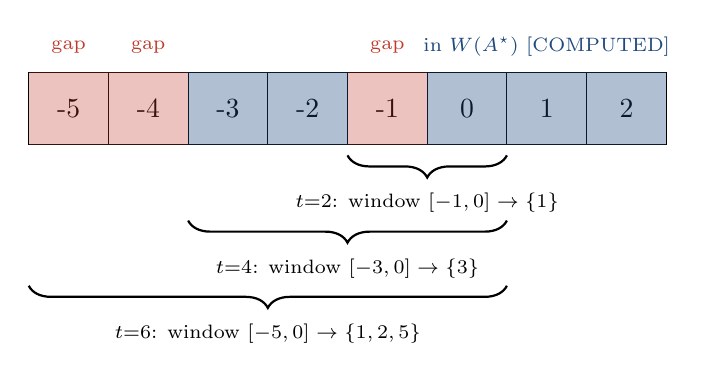
\begin{tikzpicture}[scale=0.92]
    \definecolor{shadow}{RGB}{31,73,125}
    \definecolor{gap}{RGB}{192,57,43}
    % cells -5..2
    \foreach \x/\lab in {-5/-5,-4/-4,-3/-3,-2/-2,-1/-1,0/0,1/1,2/2} {
      \draw (\x*1.1,0) rectangle ++(1.1,1);
      \node at (\x*1.1+0.55,0.5) {\lab};
    }
    % W members filled: -3,-2,0,1,2 ; gaps: -5,-4,-1
    \foreach \x in {-3,-2,0,1,2} {
      \fill[shadow,opacity=0.35] (\x*1.1,0) rectangle ++(1.1,1);
    }
    \foreach \x in {-5,-4,-1} {
      \fill[gap,opacity=0.30] (\x*1.1,0) rectangle ++(1.1,1);
      \node[gap] at (\x*1.1+0.55,1.35) {\scriptsize gap};
    }
    \node[shadow] at (1.65,1.35) {\scriptsize in $W(A^\star)$ [COMPUTED]};
    % brackets for test windows [1-t,0]: t=2 -> [-1,0], t=4 -> [-3,0], t=6 -> [-5,0]
    \draw[decorate,decoration={brace,mirror,amplitude=8pt},thick]
      (-1*1.1,-0.15) -- (0*1.1+1.1,-0.15)
      node[midway,below=10pt] {\scriptsize $t{=}2$: window $[-1,0]\to\{1\}$};
    \draw[decorate,decoration={brace,mirror,amplitude=8pt},thick]
      (-3*1.1,-1.05) -- (0*1.1+1.1,-1.05)
      node[midway,below=10pt] {\scriptsize $t{=}4$: window $[-3,0]\to\{3\}$};
    \draw[decorate,decoration={brace,mirror,amplitude=8pt},thick]
      (-5*1.1,-1.95) -- (0*1.1+1.1,-1.95)
      node[midway,below=10pt] {\scriptsize $t{=}6$: window $[-5,0]\to\{1,2,5\}$};
  \end{tikzpicture}
  \caption{The sliding shadow window of Theorem~\ref{thm:march} for
    $A^\star$ near the bottom edge ($[1,184]\subseteq W(A^\star)$ by
    saturation, so cells $1,2$ are filled). As $t$ grows, the test
    window $[1-t,0]$ slides left through the fixed shadow; each gap it
    frames becomes a hole at $g+t$. The fixed gap $-1$ generates the
    traveling hole $\{1\},\{2\},\{3\}$ at $t=2,3,4$; the deeper gaps
    $-4,-5$ enter at $t=5,6$. Shadow membership is [COMPUTED]
    $\times2$; the hole values are forced by~\eqref{eq:marchpos}.}
  \label{fig:window}
\end{figure}

\subsection{The corrected chain and $\psi$-identities}
\label{sec:chain}

R234's hostile review demoted two R227 claims to [OPEN]:
Corollary~1's chain/width framing (``maximal saturated translation
interval'', width $\lambda+\eta+1$) omitted the containment
$A+t\subseteq[1,N]$ --- the reviewer's $N=2$, $A=\{1,2\}$ toy admits
$\{0,1\},\{2,3\}$, both outside $[1,2]$ --- and Theorem~2's ``both
chain translations'' assertion is false as stated
($\mathrm{holes}(\varphi(A^\star)-2)=\{184\}$)
\cite{D234,D235}. The corrected statements, which passed hostile
re-review \cite{D238}, are:

\begin{theorem}[$\psi$-translate identities; PROVED \cite{D246}]
  \label{thm:psi}
  For all $S,c$: $\psi_c(S)=\varphi(S)-(185-c)$ as sets; hence
  $\psi_{184}(A^\star)=\varphi(A^\star)-1$ and, with the [COMPUTED]
  premise $E_4=A^\star-1$, $\psi_{182}(E_4)=\varphi(A^\star)-2$.
  Both are translates of $\varphi(A^\star)$ --- the chain-membership
  wording is dropped. Distinguishing [COMPUTED] fact:
  $\mathrm{holes}(\varphi(A^\star)-1)=\emptyset$,
  $\mathrm{holes}(\varphi(A^\star)-2)=\{184\}$.
  (Lean: \url{CorrectedMarch.psi_as_phi_translate},
  \url{psi184_translate}, \url{psi182_E4}.)
\end{theorem}

\begin{corollary}[Saturated chain with containment; PROVED \cite{D246}]
  \label{cor:chain}
  For saturated Sidon $A\subseteq[1,N]$, $m=\min A$, $M=\max A$,
  integer runs $\lambda,\eta$ as in~\eqref{eq:lambdaruns}, and
  $t\in\mathbb{Z}$:
  \begin{equation}
    \label{eq:chainbounds}
    \text{saturated}(A+t)\iff
      \max(-\eta,1-m)\le t\le\min(\lambda,N-M),
  \end{equation}
  \begin{equation}
    \label{eq:chainwidth}
    \text{width}=\min(\lambda,N-M)+\min(\eta,m-1)+1,
  \end{equation}
  the old shadow range intersected with the feasibility range
  $1-m\le t\le N-M$ (Lean: \texttt{CorrectedMarch.feas\_iff}).
  The chain is non-empty ($t=0$ always qualifies).
  (Lean: \url{CorrectedMarch.chain_bounds},
  \url{CorrectedMarch.chain_width},
  \url{CorrectedMarch.chain_zero_mem}.)
\end{corollary}
\noindent Instantiation [COMPUTED] $\times2$ \cite{D235}:
$A^\star\to[0,1]$ width~2; $\varphi(A^\star)\to[-1,0]$ width~2;
$C=E_3-2\to[0,0]$ width~1 --- matching the old chains here, now with
the containment proof. The reviewer's $N=2$ toy: the corrected formula
gives bounds $[0,0]$, width~1, confirmed by brute force; the old
formula's claimed width~3 was wrong there. The old framings (without
containment; ``both chain translations'') stay superseded and [OPEN].

\subsection{The unsaturated march}
\label{sec:unsat}

R233 proved the march for \emph{any} Sidon $A$, no saturation assumed
\cite{D233}. R238's hostile review refuted it \emph{as stated}: the
empty set is Sidon and is not excluded, and for $N=184$, $A=\emptyset$,
$t=185$ the proof's step
$S_2=\{p:p-t<1\}=[1,t]$ drops the $p\in[1,N]$ restriction, wrongly
including $185$ as a hole (the symmetric $t=-185$ step wrongly
includes $0$) \cite{D238}. The corrected re-review SURVIVED
\cite{D246}; the fix is one line --- an explicit $A\ne\emptyset$
hypothesis, which forces $1-N\le t\le N-1$ from $A+t\subseteq[1,N]$,
making the dossier's unclipped edge terms exact.

\begin{theorem}[Unsaturated Translation March; PROVED \cite{D250}]
  \label{thm:unsat}
  Let $A\subseteq[1,N]$ be Sidon, $A\ne\emptyset$, $t$ with
  $A+t\subseteq[1,N]$. With $\mathrm{edge}_t$ the saturated term of
  Theorem~\ref{thm:march},
  \begin{align}
    \label{eq:unsatpos}
    t\ge0:\quad \mathrm{holes}(A+t)
      &= \bigl((\mathrm{holes}(A)+t)\cap[1,N]\bigr)\;\sqcup\;
        \{p\in[1,t]:p-t\notin W(A)\}, \\
    \label{eq:unsatneg}
    t\le0:\quad \mathrm{holes}(A+t)
      &= \bigl((\mathrm{holes}(A)+t)\cap[1,N]\bigr)\;\sqcup\;
        \{p\in[N+t+1,N]:p-t\notin W(A)\}.
  \end{align}
  The union is disjoint. Saturation recovery: $\mathrm{holes}(A)=\emptyset$
  kills the propagation term and~\eqref{eq:unsatpos} reduces to
  Theorem~\ref{thm:march}.
  (Lean: \texttt{TranslationMarchUnsat.march\_unsat\_pos/neg},
  \texttt{march\_unsat\_disjoint\_pos/neg}, with the
  \url{A.Nonempty} fix.)
\end{theorem}

\begin{corollary}[Propagation, rescue, additive bound; PROVED \cite{D250}]
  \label{cor:unsat}
  (i) \emph{Conveyor:}
  $(\mathrm{holes}(A)+t)\cap[1,N]\subseteq\mathrm{holes}(A+t)$ always;
  new holes enter only at the near edge, old holes exit only off the
  far edge (\url{propagation_subset}).
  (ii) \emph{Rescue threshold:} for $t\ge0$,
  $\mathrm{holes}(A)\ne\emptyset$:
  \begin{equation}
    \label{eq:rescue}
    (\mathrm{holes}(A)+t)\cap[1,N]=\emptyset \iff t>N-\min(\mathrm{holes}(A)),
  \end{equation}
  past which the march is pure saturated-march form (symmetric:
  $t<1-\max(\mathrm{holes}(A))$ for $t\le0$)
  (\texttt{rescue\_threshold\_pos/neg}).
  (iii) \emph{Additive bound:}
  \begin{equation}
    \label{eq:additive}
    |\mathrm{holes}(A+t)|\le|\mathrm{holes}(A)|+|t|,
  \end{equation}
  both terms bounded, disjoint
  (\texttt{additive\_bound\_pos/neg}).
\end{corollary}

The naive extension fails honestly: the saturated bound
$|\mathrm{holes}|\le|t|$ does \emph{not} generalize ---
$A_0=[61,62,65,73,88,119,121,143,160]$ at $t=1$ has $4$ holes
$\{1,13,53,154\}$ (propagation $\{13,53,154\}$ + edge $\{1\}$), and
the additive bound $3+1=4$ is sharp there \cite{D233}.
Rescue observed live [COMPUTED] $\times2$, $450/450$ march entries
\cite{D233}: $F_{4b}=[61,62,68,79,88,109,111,121,166]$ (holes
$\{179,182\}$) rescues at $t>5$: $1\!\to\!\{1,180,183\}$,
$6\!\to\!\{1,\dots,6\}$ pure edge; $F_{5a}$ rescues at $t>14$;
$F_{4a}$ at $t>24$.

\subsection{Hole-twin dips}
\label{sec:dip}

R228's witness $A_{0w1}-5=[7,56,60,68,83,99,116,118,123]$ sharing
$S_1$'s blocked set (holes $\{170,182\}$, neither on a saturated chain)
refuted ``sharing requires saturated-chain membership''
\cite{D231}. The dip theorem turns this into a predictive sufficient
condition. R238's hostile review refuted the original statement on two
points \cite{D238}: (1) the hole-twin definition requires \emph{two
Sidon $9$-sets} but the theorem assumed only ``Sidon'' --- countermodel
$A=\{1\}$, $S=\{101\}$ with a doctored $W$ satisfying every stated
hypothesis, but no nine-element sets anywhere; (2) the S1 corollary
cited P3 for $S_1$'s hole set, which P3 never states. The corrected
statement carries explicit $9$-set hypotheses and explicit S1 premises;
its hostile re-review SURVIVED \cite{D246}.

\begin{theorem}[Hole-twin dip; PROVED \cite{D250}]
  \label{thm:dip}
  Let $A\subset[1,184]$ be a Sidon $9$-set with
  $C_{\max}:=\mathrm{maxcov}(\mathrm{chain}(A))\le183$. Let
  $g_1<g_2$ be consecutive shadow gaps of $W(A)$. If valid $t^\star$
  has $[1-t^\star,184-t^\star]\cap\mathrm{gaps}(W(A))=\{g_1,g_2\}$
  (clean window), then $W^\star=A+t^\star$ is a Sidon $9$-set with
  $\mathrm{holes}(W^\star)=\{g_1+t^\star,g_2+t^\star\}$
  ($\mathrm{cov}(W^\star)=182$); if $S\ne W^\star$ is a Sidon $9$-set
  with the same holes and $\mathrm{maxcov}(\mathrm{chain}(S))<184$,
  then $(S,W^\star)$ are hole-twins; if $C_{\max}=183$ then $W^\star$
  sits below the chain maximum (``chain dip'').
  (Lean: \url{HoleTwinDip.dip_holes},
  \url{dip_blocked_eq}, \url{chain_translate},
  \url{maxcov_translate}, \url{hole_twin_of_dip},
  \url{chain_dip}.)
\end{theorem}

\noindent\textit{S1 instance} [PROVED as \url{HoleTwinDip.s1_instance};
shadow/gap data [COMPUTED] $\times2$ as explicit hypotheses]
\cite{D240,D250}: the base is $A=\mathrm{FW183}\#5=
[12,61,65,73,88,104,121,123,128]$ (attribution correction: R231's P3
labeled the \emph{dip target} $W^\star=A-5=[7,56,60,68,83,99,116,118,123]$
as ``$A_{0w1}$''; the dip anatomy belongs to the true base
\cite{D240}; the Lean instance's first parameter name retains the old
label but its gap data are those of $[12,61,65,73,88,104,121,123,128]$).
$\mathrm{gaps}(W(A))\cap[150,200]=\{175,187,192,193,194\}$ (consecutive
$175,187$, spacing $12$); $t^\star=-5$, window $[6,189]$ clean
$\to$ holes $\{170,182\}=\mathrm{holes}(S_1)$ for
$S_1=[47,66,70,80,82,102,110,139,144]$; chain maxcovs $183$/$182$;
$(S_1,W^\star)$ are hole-twins at a chain dip ($182<183$).

R240 generalized the theorem to an arbitrary clean gap set $G$
(one or more gaps; the exact clean-window equality already forces $G$
consecutive and finite) [PROVED*] \cite{D240}. Its $|G|=1$ instance:
$A_1=\varphi(\mathrm{FW183}\#5)=[57,62,64,81,97,112,120,124,173]$,
clean window $[0,183]\cap\mathrm{gaps}=\{10\}$, $t^\star=1$,
$W^\star=[58,63,65,82,98,113,121,125,174]$ with holes $\{11\}$;
$A_{183}=[18,62,63,79,88,111,119,121,125]$ has the same holes, so
$(A_{183},W^\star)$ are hole-twins at the chain maximum ($183=183$,
not a dip) --- the mechanism generalizes; genuine below-max dips need
$|G|\ge2$ \cite{D247}. As a prediction engine the generalization
scored $34/34$ verified single-gap anchors across $9$ bases and $15$
new hole-twin pairs [COMPUTED] $\times2$ \cite{D243}; the pairing
logic for these is [PROVED*] (R240), their anchors [COMPUTED], and $22$
anchors found no catalog partner (partners are contingent, not
forced).

\subsection{Dip-march mechanics}
\label{sec:dipmarch}

For the window gap sets $G_t=I_t\setminus W$ ($I_t=[1-t,184-t]$), the
step-to-step evolution is pure combinatorics --- no hypotheses on $W$
at all:

\begin{theorem}[Dip-march; PROVED \cite{D262}]
  \label{thm:dipmarch}
  For all $t\in\mathbb{Z}$:
  \begin{equation}
    \label{eq:slide}
    G_{t+1}=(G_t\setminus\{184-t\})\cup E_t,\qquad
    E_t=\{-t\}\ \text{if }{-t}\notin W\text{ else }\emptyset
  \end{equation}
  (Lean: \texttt{DipMarch.sliding\_window\_up/down}).
  If $G_t=\{g\}$ and $G_{t+1}=\{g'\}$ are both clean single-gap, then
  $g'=g$ or $g=184-t$ (\texttt{same\_gap\_persistence}). Moreover
  \begin{equation}
    \label{eq:cont}
    G_{t+1}=\{g\}\iff g\le183-t\ \text{AND}\ {-t}\in W,
  \end{equation}
  with three exhaustive, exclusive non-continuation cases:
  (a) \emph{break:} $g\le183-t$, $-t\notin W\to G_{t+1}=\{g,-t\}$
  (holes $\{h_t+1,1\}$) (\texttt{break\_case});
  (b) \emph{reset:} $g=184-t$, $-t\notin W\to G_{t+1}=\{-t\}$
  (hole $\{1\}$) (\texttt{reset\_case});
  (c) \emph{perfect:} $g=184-t$, $-t\in W\to G_{t+1}=\emptyset$
  (no holes) (\url{perfect_case}).
  Downward dual symmetric (\url{continuation_iff_down}).
  $\varphi$-duality: $W(\varphi(A))=185-W(A)$, hence
  \begin{equation}
    \label{eq:dual}
    G_t(\varphi(A))=\{185-g:g\in G_{-t}(A)\}
  \end{equation}
  (Lean: \url{DipMarch.phi_duality}).
\end{theorem}

Verification [COMPUTED] $\times2$ \cite{D247}: the recurrence at
$3482/3482$ window steps over $47$ $\varphi$-bases; $24/24$ boundary
classifications exact, including every exotic case ---
$\varphi(\#5\,A_{0w1})$ breaks up ($t=2\to3$) and down ($t=-8\to-9$),
$\varphi(\#1\,W_{183})$ runs the full lifecycle
march $\to$ edge-exit $\to$ perfect translate (holes $\emptyset$)
$\to$ reset; $\varphi$-duality $3529/3529$. The hole-reading corollary
(constant-gap run $\implies$ holes march $1$ per step) is conditional
on Theorem~\ref{thm:dip}'s premises and remains OUT OF SCOPE of the
Lean module, pending the R240 generalization's formalization
\cite{D258,D262}.

Forced vs.\ data, corrected \cite{D262}: given the gap landscape of
$W$, everything about how a march evolves is forced by
Theorem~\ref{thm:dipmarch} --- same-gap $\implies$ marching holes,
the exact continuation/break/reset criterion, the dual march. The gap
landscape itself is data. The R254 review corrected an overstatement:
the $11$-step run on $\varphi(\#5\,A_{0w1})$ ($t=-8\ldots+2$, gap
$\{10\}$, holes $\{2\ldots12\}$ [COMPUTED] $\times2$) is not established
by the edge memberships $\{-1,\dots,8\}\subseteq W$, $-2,193\notin W$
alone --- the reviewer exhibits an explicit Sidon $9$-set
$B=\{11,30,50,53,58,60,75,84,96\}$ ($45$ pair sums distinct) whose
shadow contains $[-1,8]$ and excludes $-2,193$ yet has interior gaps
$125,128$ in every window $-8\le t\le2$, so none of its windows is
single-gap. A clean run needs the full gap landscape as datum, not
just the edge memberships.

Table~\ref{tab:variants} summarizes the march variants, their bounds,
and their labels.

\begin{table}[t]
  \centering
  \caption{The march variants: hypotheses, hole description, bound,
    and honesty label. ``Seed'' = unsaturated starting set.}
  \label{tab:variants}
  \begin{tabular}{lllll}
    \toprule
    variant & hypotheses & hole description & bound & label \\
    \midrule
    saturated march (Thm.~\ref{thm:march})
      & saturated Sidon, $A+t\subseteq[1,184]$
      & shadow gaps in $[1-t,0]$
      & $|\mathrm{holes}|\le|t|$ & [PROVED] \\
    unsaturated march (Thm.~\ref{thm:unsat})
      & Sidon, $A\ne\emptyset$, $A+t\subseteq[1,184]$
      & rigid conveyor + edge term
      & $|\mathrm{holes}|\le|\mathrm{holes}(A)|+|t|$ & [PROVED] \\
    hole-twin dip (Thm.~\ref{thm:dip})
      & Sidon $9$-sets, clean window
      & $|G|$ framed gaps
      & $\mathrm{cov}=184-|G|$ & [PROVED] ($|G|=2$) \\
      & & & & [PROVED*] (general $G$) \\
    corrected chain (Cor.~\ref{cor:chain})
      & saturated Sidon, $m=\min A$, $M=\max A$
      & chain $[\max(-\eta,1-m),\min(\lambda,184-M)]$
      & width~\eqref{eq:chainwidth} & [PROVED] \\
      &&& (old framing) & [OPEN] \\
    dip-march mechanics (Thm.~\ref{thm:dipmarch})
      & none (pure combinatorics)
      & recurrence~\eqref{eq:slide} + break/reset
      & deterministic & [PROVED] \\
    \bottomrule
  \end{tabular}
\end{table}

%======================================================================
\section{Discussion}
%======================================================================

\paragraph{Significance.} The five modules constitute the first
machine-checked structural theory of translation marches in the
program's blocked-set framework: rigidity, the saturated and
unsaturated marches, the corrected chain/$\psi$ calculus, the dip
theorem, and the window mechanics are all exit-0 in Lean with standard
axioms only. The $11$-step dip march, the $34/34$ anchor predictions,
and the $15$ new hole-twin pairs are the theory's predictive face;
the $24/24$ break/reset classifications are its exact face. The
march form is general; the hole values are shadow data; the mechanics
are forced; the landscape is data.

\paragraph{The review gate works.} Three of the claims entering this
paper failed as stated --- all on statement-level overgeneralization
(empty set admitted; $9$-set cardinalities assumed; containment
dropped; chain membership asserted for an unsaturated translate),
never on the core mathematics, which survived in every case. Each was
restored by a one-line-class fix (explicit $A\ne\emptyset$; explicit
$|A|=|S|=9$; the feasibility intersection; translates-not-chain-members
wording), re-reviewed, and machine-checked. We also record two
prose-level corrections the reviewers caught before they could
calcify: the ``A0w1'' attribution (the dip target, not the base) and
the forced-vs-data overstatement (edge memberships do not establish a
clean run). Presenting the corrected theorems without this history
would mislead; the history is the evidence that the gate is load-bearing.

\paragraph{Limitations and [OPEN] items.} (i) All instantiations are
[COMPUTED]: shadow tables, march tables ($65/65$, $450/450$), and the
$15$ pairs rest on exact computation, not deduction. (ii) The R240
arbitrary-gap generalization and its pairing logic are [PROVED*],
not formalized; the S1 instance is the two-gap [PROVED] case.
(iii) R247's hole-reading corollary (constant-gap run $\implies$
marching holes) is out of the Lean module's scope \cite{D262}.
(iv) Why chains' shadow gaps align across chains (e.g.\ $A^\star$'s
chain at $t=3$ and $C$'s at $s=2$ both yielding $\{2\}$) remains
[OPEN] --- the remaining data-specific mystery \cite{D227}. (v) The
old R227 chain/width framing and ``both chain translations'' assertion
stay [OPEN] as stated. (vi) Necessity of saturated-chain membership
for sharing is untouched (R228's target) \cite{D227}.

%======================================================================
\section{Conclusion}
%======================================================================

We have proved and machine-checked the translation-march theory:
rigidity (Lemma~\ref{lem:rigidity}), the saturated march
(Theorem~\ref{thm:march}), the saturation iff-core
(Corollary~\ref{cor:iffcore}), the corrected chain and $\psi$
calculus (Theorem~\ref{thm:psi}, Corollary~\ref{cor:chain}), the
unsaturated march with its sharp additive bound
(Theorem~\ref{thm:unsat}, Corollary~\ref{cor:unsat}), the hole-twin
dip theorem with its S1 instance (Theorem~\ref{thm:dip}), and the
dip-march window mechanics with $\varphi$-duality
(Theorem~\ref{thm:dipmarch}) --- all [PROVED] in five Lean modules
with exit-0 builds and standard-only axioms. Along the way the
hostile-review gate refuted three claims as stated; each was repaired
with a minimal hypothesis fix and restored machine-checked, and the
correction history is part of the record. The natural next steps are
formalizing the R240 arbitrary-gap generalization, a theory of the
cross-chain shadow-gap alignment that remains [OPEN], and the march
graph of break/reset cascades suggested by the dip-march lifecycle.

%======================================================================
\section{References}
%======================================================================

\begin{thebibliography}{99}

\bibitem{ET41}
P.~Erd\H{o}s and P.~Tur\'an,
\emph{On a problem of Sidon in additive number theory, and on some
related problems},
J. London Math. Soc.\ \textbf{16} (1941), 212--215.

\bibitem{D201}
D.~Blair,
\emph{Unsolved Math --- Round 201: blocked-set framework},
program dossier, 2026-10.
(Supplied datum: $B(A)$, puncture definitions.)

\bibitem{D213}
D.~Blair,
\emph{Unsolved Math --- Round 213: puncture machinery},
program dossier, 2026-10.
(Supplied datum: blocked-set framework, puncture theory.)

\bibitem{D215}
D.~Blair,
\emph{Unsolved Math --- Round 215: reflection equivariance},
program dossier, 2026-10.
(Supplied datum: $\varphi$-equivariance of the blocked set.)

\bibitem{D227}
D.~Blair,
\emph{Unsolved Math --- Round 227: R224's Translation March proved
structurally},
program dossier, 2026-10-09.
(Supplied datum: Lemma~1, Theorem~1, Corollaries~1--3, Theorem~2,
shadow tables, march tables $|t|\le6$, $65/65$ checks.)

\bibitem{D231}
D.~Blair,
\emph{Unsolved Math --- Round 231: hole-twin dip theorem [PROVED*]},
program dossier, 2026-10-09.
(Supplied datum: hole-twin definition, dip theorem, S1 instance,
$40$-center hunt.)

\bibitem{D233}
D.~Blair,
\emph{Unsolved Math --- Round 233: generalized Translation March for
unsaturated seeds},
program dossier, 2026-10-09.
(Supplied datum: unsaturated march theorem, propagation/rescue/
additive-bound corollaries, six seed march tables, $450/450$ checks.)

\bibitem{D234}
D.~Blair,
\emph{Unsolved Math --- Round 234: Lean lane --- R227 review gate and
\url{TranslationMarch.lean}},
program dossier, 2026-10-09.
(Supplied datum: hostile-review verdicts, demotions, Lean
verification of the surviving core.)

\bibitem{D235}
D.~Blair,
\emph{Unsolved Math --- Round 235: R234's two demotions restored
(corrected statements)},
program dossier, 2026-10-09.
(Supplied datum: corrected Theorem~2* and Corollary~1* proofs,
instantiations, $N=2$ toy.)

\bibitem{D238}
D.~Blair,
\emph{Unsolved Math --- Round 238: Lean lane --- R233/R231/R200/R235
review gates},
program dossier, 2026-10-09.
(Supplied datum: empty-set and singleton refutations verbatim,
R235 re-review verdicts.)

\bibitem{D240}
D.~Blair,
\emph{Unsolved Math --- Round 240: generalized hole-twin dip theorem},
program dossier, 2026-10-10.
(Supplied datum: arbitrary-gap generalization, S1/A183 instances
with corrected attribution.)

\bibitem{D243}
D.~Blair,
\emph{Unsolved Math --- Round 243: single-gap clean-window hole-twin
hunt},
program dossier, 2026-10-10.
(Supplied datum: $34/34$ anchor predictions, $15$ new hole-twin
pairs, $\times2$ paths.)

\bibitem{D246}
D.~Blair,
\emph{Unsolved Math --- Round 246: Lean lane ---
\url{CorrectedMarch.lean} and the two re-reviews},
program dossier, 2026-10-10.
(Supplied datum: corrected-module verification, audit of draft
``Checked'' headers, re-review transcripts.)

\bibitem{D247}
D.~Blair,
\emph{Unsolved Math --- Round 247: the dip-march theorem},
program dossier, 2026-10-10.
(Supplied datum: sliding-window mechanics, $\varphi$-duality,
forced-vs-data separation, $3482/3482$ and $3529/3529$ checks.)

\bibitem{D250}
D.~Blair,
\emph{Unsolved Math --- Round 250: Lean lane --- repair and formalize
three review-cleared drafts},
program dossier, 2026-10-10.
(Supplied datum: \url{TranslationMarchUnsat.lean} and
\url{HoleTwinDip.lean} repair + verification.)

\bibitem{D258}
D.~Blair,
\emph{Unsolved Math --- Round 258: Lean lane --- \url{DipMarch.lean}
repaired, R245 review launched},
program dossier, 2026-10-10.
(Supplied datum: DipMarch elaboration-error repairs, bakkie exit~0,
nine-theorem axiom audit.)

\bibitem{D262}
D.~Blair,
\emph{Unsolved Math --- Round 262: Lean lane ---
\url{DipMarch.lean} close-out},
program dossier, 2026-10-10.
(Supplied datum: \url{DipMarch.lean} verification, R254 reviewer's
forced-vs-data correction, scope notes.)

\end{thebibliography}

\end{document}

% WEAKNESSES (substantive, noticed while drafting):
% W1. The paper never defines or exhibits the blocked-set framework's primitive
%     B(A)/W(A) computational content for any set other than Astar's shadow near
%     the edges: every figure, table, and worked example is Astar- or
%     F4b-flavored, so the "general N" claim of the theorems is illustrated only
%     by the saturated/unsaturated dichotomy, not by a genuinely different
%     structure (e.g. a march on a non-[1,184] universe or a non-Sidon seed).
% W2. The S1 instance's corrected attribution (true base FW183#5 vs the
%     parameter name "A0w1" retained in HoleTwinDip.s1_instance) is flagged in
%     prose but the paper cannot fix the Lean parameter name without a module
%     edit; a reader checking the module sees the old label and must trust the
%     prose that the [COMPUTED] gap hypotheses are the corrected ones.
% W3. Theorem 5's hole-reading corollary is stated as conditional on R240(i) and
%     left out of the Lean module's scope; the paper's narrative still leans on
%     "holes march 1 per step" in the forced-vs-data discussion, which is the
%     one place where the [PROVED] mechanics and the [PROVED*] interpretation
%     are not visually separated for the reader.
% TYPOGRAPHY ISSUES (noticed while drafting):
% T1. In Figure 1, the three brace decorations are stacked at fixed offsets
%     (-0.15, -1.05, -1.95) and will collide with the caption if the figure is
%     rescaled; the offsets should be computed from the brace amplitude instead
%     of hardcoded.
% T2. Table 1's two-line cells (hole-twin dip split across "[PROVED] (|G|=2)" /
%     "[PROVED*] (general G)" rows) break the row-height rhythm; a single
%     multirow cell would align the variant column properly.
% T3. Theorem/corollary environments number continuously across sections
%     (Lemma 1, Theorem 2, ...) while the text cross-references them by both
%     number and name; a reader jumping from "Theorem 5" in the Discussion to
%     the Results section must scan past unrelated numbers --- per-section
%     numbering (e.g. \numberwithin{theorem}{section}) would be kinder.
